\section{Fluxional execution model} \label{section:model}

% The compiler we present in section \ref{section:compiler} focuses on web applications that tend to follow the functional paradigm while keeping a global memory.
% Such applications are built using functions that are executed sequentially to assure the exclusivity of access on the global memory.
% This is a serious performance issue, as it avoids to leverage the parallelism of modern architectures.

% We present in this section a different execution model that isolates the memory accessible to some functions.
% This approach allows to execute these functions in parallel, hence, to benefit of the performance improvements of this parallelism.
% This execution model is close to the actor model, as the function are executed on autonomous execution units with their own isolated memory, communicating by messages.

% In this section, we present an execution model to allow the execution of functions in parallel of a main thread.
% Each parallel function is encapsulated in an autonomous execution container with its own memory.

In this section, we present an execution model to provide scalability to web applications.
% The execution of functions may dynamically be reallocated at run time depending on the load of servers.
Functions are encapsulated in an autonomous execution container with their own state, so as to be reallocated, and executed in parallel.
This execution model is similar to the actors model, as the execution container are independent and communicate by messages.
Though the communications are assimilated to stream of messages, similarly to the data-flow programming model.
It allows to reason on the throughput of these streams, and to react to load increases.
% As we focus on real-time web applications, the streams of message correspond to the input stream of requests.

% This execution model is also close to the functional paradigm, as the execution container contains function to execute at each message reception.
% The function receives parameters from the input message, and sends one, or more, output streams of messages to other execution container.

In the following paragraphs, we present the autonomous containers.
Then we present the messaging system to carry the communication between these execution containers.
Finally, we present an example application using this execution model.

\subsection{Fluxions}

The fluxional execution model manages and invokes autonomous execution containers named fluxion $\bnfpn{flx}$.
A fluxion is composed of a unique name $\bnfpn{id}$, a processing function $\bnfpn{fn}$, and a local memory called a \textit{context} $\bnfpn{ctx}$.
Its function $\bnfpn{fn}$ consumes an input stream $\bnfpn{stream}$ and generates one or more outputs streams to other fluxions $\bnfpn{dest}$.
The \textit{context} handles the state on which a fluxion relies between two message receptions.
At a message reception, the fluxion modifies its \textit{context}, and sends back messages to downstream fluxions.
A message is composed of the recipient fluxions' names and a body.

The \textit{context} of a fluxion might be shared with other fluxions.
Fluxions depending upon the same states are grouped.
Each fluxion is associated with one or more tags to express these dependencies.
If we can consider the fluxion names as the graph of data communications, then we can consider these tags as the graph of state communications.
To assure the consistency of the states, all the fluxions of a group access the state in a mutual exclusion fashion.
They are all executed sequentially.

Fluxions are executed on an event-loop with an isolated heap ; it is a \textit{Node.js} instance.
The event-loop assures the exclusivity of operations on the heap.
Only one fluxion is executed at once on the event-loop.
Consequently, the more fluxions on an event-loop, the less time fraction each fluxion has for its execution.
That is why we propose to stretch the execution of an application by distributing the fluxions on different event-loop.
This distribution is based on the dependencies between fluxions.


% A fluxion receiving and sending heap reference can be stateless, hence replicated.
% However, because it share references, it needs to be on the same group than other another fluxions (think about req / res).
% If all the fluxion of a group are stateless, they can be replicated exactly like if it was a single fluxion. 







We represent here the syntax of a high-level language to represent a program in the fluxionnal form.
It is the target for our compiler.
\begin{bnf*}
  \bnfprod{program}    {\bnfpn{flx} \bnfor \bnfpn{flx} \bnfsp \bnftd{eol} \bnfsp \bnfpn{program}}\\
  \bnfprod{flx}        {\bnfts{\texttt{flx}} \bnfsp \bnfpn{id} \bnfsp \bnfpn{tags} \bnfsp \bnfpn{ctx} \bnfsp \bnftd{eol} \bnfsp \bnfpn{streams} \bnfsp \bnftd{eol} \bnfsp \bnfpn{fn}}\\
  % \bnfprod{tags}       {\bnfts{\bnfpn{id}} \bnfor \bnfpn{id} \bnfsp \bnftd{eol} \bnfsp \bnfpn{tags} \bnfor \bnftd{empty string}}\\
  \bnfprod{tags}       {\bnfts{\texttt{\&}} \bnfpn{list} \bnfor \bnftd{empty string}}\\
  \bnfprod{streams}    {\bnfts{\texttt{null}} \bnfor \bnfpn{stream} \bnfor \bnfpn{stream} \bnfsp \bnftd{eol} \bnfsp \bnfpn{streams}}\\
  \bnfprod{stream}     {\bnfpn{op} \bnfsp \bnfpn{dest} \bnfsp [\bnfpn{msg}]}\\
  \bnfprod{dest}       {\bnfpn{list}}\\
  \bnfprod{ctx}        {\bnfts{\texttt{\{}} \bnfpn{list} \bnfts{\texttt{\}}}}\\
  \bnfprod{msg}        {\bnfts{\texttt{[}} \bnfpn{list} \bnfts{\texttt{]}}}\\
  \bnfprod{list}       {\bnfpn{id} \bnfor \bnfpn{id} \bnfsp \bnfts{,} \bnfsp \bnfpn{list}}\\
  \bnfprod{op}         {\bnfts{\texttt{>}\texttt{>}} \bnfor \bnfts{\texttt{-}\texttt{>}}}\\
  \bnfprod{id}         {\bnftd{Javascript identifier}}\\
  \bnfprod{fn}         {\bnftd{Javascript and stream syntax}}\\
\end{bnf*}
\vspace{-2.5\baselineskip}


\subsection{Messaging system}

% In a distributed approach, the messages between fluxions would be carried over a distributed message broker.
% However this execution model is only a simulation of a distributed execution environement.
% We simplify the distributed message broker with a master message queue to centralize communication between workers, though, each worker has its own local message queue.
% The messaging system is the core of the execution model.
% It carries messages and invokes fluxions at reception.
% The messaging system sends messages to the worker hosting the destination fluxion.
% Locally, the master worker hosts fluxions that need access to the external network or the global memory.
% Using a message queue allows to execute multiple processing chains fairly and concurrently, without difference in scheduling local messages, or network messages.

The messaging system assures the stream communications between fluxions.
It carries messages based on the names of the recipient fluxions, so every fluxion needs to be registered with a unique name.
The messages are queued for the event-loop to execute the associated fluxions sequentially.
The messaging system allows the execution to be distributed on several event-loop.
Each event-loop executes a group of fluxion with dependencies on the same state.
An event-loop is isolated from the other event-loops.
The messaging-system carries messages from one event-loop to the other, and assure that the message is queued on the event-loop executing the destination fluxion.

% If two fluxions share the same name, it would lead to a conflicting situation for the messaging system.

% This registration associates a processing function with a unique name and an initial \textit{context}.
% The registration is done by calling \texttt{register(<name>, <fn>, <context>)}, \circled{1}.
% A fluxion can dynamically register other fluxions

The execution cycle of a fluxional application is illustrated in figure \ref{fig:MesSys}.
Circles represent registered fluxions.
The fluxion \textit{reply} has a context containing the variable \texttt{count}.
The plain arrows represent the actual message paths in the messaging system, while the dashed arrows between fluxions represent the message streams as seen in the fluxionnal application.
The streams between workers are serialized.

\begin{figure}[h!]
  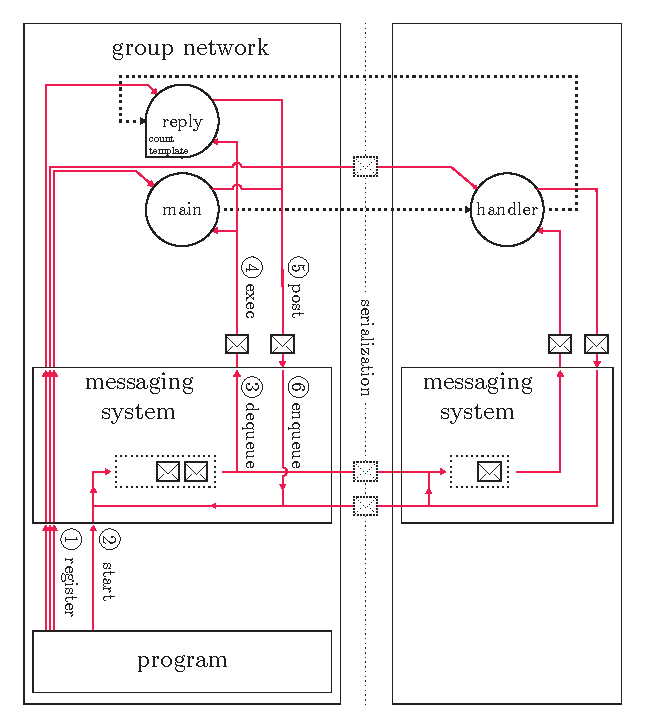
\includegraphics[width=\linewidth]{ressources/schema-message.pdf}
  \caption{The fluxionnal execution model in details}
  \label{fig:MesSys}
\end{figure}

When a new request is received, a \texttt{start} message triggers the flow, \circled{2}. %  using the function \texttt{start(<msg>)}
This first message represents the incoming of a request from a user.
The system dequeues this message and dispatch it to the destination fluxion, \textit{handler}, \circled{3} and \circled{4}.
The fluxion \textit{handler} sends back a message, \circled{5}, to be enqueued in the centralized message queue, \circled{6}. % using the function \texttt{post(<msg>)}
The system loops through steps \circled{3} and \circled{4} until the queue is empty.
This cycle starts again for each new incoming request causing a \texttt{start} message.

% Algorithms \ref{alg:parcours} and \ref{alg:traitement} describe the behavior of the messaging system after the \texttt{start} function invocation.

% \begin{algorithm}
% \caption{Message queue walking algorithm}
% \label{alg:parcours}
% \begin{algorithmic}
% \Function{loopMessage}{\null}
% \While{$msg$ \textbf{presents in} $msgQueue$}
% \State $msg \gets$ \Call{dequeue}{\null} \Comment{\circled{3}}
% \State \Call{ProcessMsg}{$msg$}
% \EndWhile
% \EndFunction
% \end{algorithmic}
% \end{algorithm}

% \begin{algorithm}
% \caption{Message processing algorithm}
% \label{alg:traitement}
% \begin{algorithmic}
% \Function{processMsg}{$msg$}
% \For{$dest$ \textbf{in} $msg.dest$}
% \State $worker \gets lookup(dest)$
% \State \Call{worker.send}{$fluxion, msg.body$} \Comment{\circled{4}}
% % \State $message \gets$ \Call{exec}{$fluxion, msg.body$} \Comment{\circled{4} \& \circled{5}}
% % \State \Call{enqueue}{$message$} \Comment{\circled{6}}
% \EndFor
% \EndFunction
% \end{algorithmic}
% \end{algorithm}

\subsection{Service example}

To illustrate the fluxional execution model, and the compiler we present an example of a simple web application.
This application reads the file containing its own source code, and sends it back along with a request counter.

The original source code of this application is available on github\cite{flx-example}, and in listing \ref{lst:source}.
In this source code, some points are worth noticing.
The \texttt{handler} function, line 5 to 11, receives the input stream of request.
The \texttt{template} function simply format the output stream to send back to the client.
The \texttt{count} variable at line 3 increments the request counter.
This object needs to be persisted in the fluxion \textit{context}.
The \texttt{app.get} and \texttt{res.send} functions, respectively line 5 and 8, interface the application with the clients.
The processing chain of functions occurs between these two functions : $\texttt{get} \twoheadrightarrow \texttt{handler} \to \texttt{reply}$.

\begin{code}[js,
  caption={Simple web application that replies to every request with its own source code and a counter},
  label={lst:source}]
var app = require('express')(),
    fs = require('fs'),
    count = 0;

app.get('/', function handler(req, res){
  fs.readFile(__filename, function reply(err, data) {
    count += 1;
    res.send(err || template(count, data));
  });
});

app.listen(8080);
\end{code}

This application is transformed into the high-level fluxionnal language in listing \ref{lst:fluxional}, and illustred in Figure \ref{fig:MesSys}.
% We expect a similar result with the compiler described in section \ref{section:compiler}.
% Horizontal dashed lines show virtual transmission of messages between fluxions although they all go through the messaging system.

% \begin{figure}[h!]
%   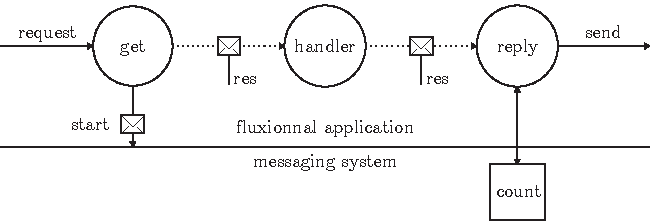
\includegraphics[width=\linewidth]{ressources/flux.pdf}
%   \caption{Fluxions chain manually extracted from the example application}
%   \label{fig:fluxions}
% \end{figure}

\begin{code}[flx, caption={Transformation of the example application in our high-level fluxional language},label={lst:fluxional}]
flx main & network
>> handler [res]
  var app = require('express')(),
      fs = require('fs'),
      count = 0;

  app.get('/', >> handler); //@\label{lst:fluxional-streamtohandler}@
  app.listen(8080);

flx handler
-> reply [res]
  function handler(req, res) {
    fs.readFile(__filename, -> reply); //@\label{lst:fluxional-readfile}@
  }

flx reply & network {count, template}
-> null
  function reply(error, data) {
    count += 1; //@\label{lst:fluxional-counter}@
    res.send(err || template(count, data)); //@\label{lst:fluxional-ressend}@
  }
\end{code}

The application is organized as follow.
The chain of fluxion starts with the fluxion \texttt{main}, continues with the fluxion \texttt{handler}, and ends with the fluxion \texttt{reply}.
The fluxions \texttt{main} and \texttt{reply} have the tag \texttt{network}.
This tag indicates their dependency over the network interface, because they  received the response from and send it back to the client.
The fluxion \texttt{handler} has no tag, it doesn't have any dependencies, and can be distributed on an isolated event-loop.

The last fluxion, \texttt{reply}, depends on its context to holds the variable \texttt{count} and the function \texttt{template}.
It also depends on the variable \texttt{res} created by the first fluxion, \texttt{main}.
This variable needs to flow through the chain of fluxion until the fluxion \texttt{reply} that depends on it.
The output streams in the chains carry the variable \texttt{res}.

It is interesting to note that if the last fluxion, \texttt{reply}, did not had a context, the group of fluxion based on the tag \texttt{network} would be stateless.
It would allow to replicate the whole group on as many event-loop as needed to cope with the incoming traffic.

This execution model allows to parallelize the execution of an application.
Hence, it improves the scalability of the application.
Fluxions can be distributed on different event-loop, hence executed in parallel. As a fluxion contains its state and expresses its dependencies, it can migrate accordingly.
Fluxions with no state could be replicated to make data parallelism, additionally to the pipeline parallelism.

Our goal, as described in the introduction, is not to propose a new programming paradigm with this high-level language but to automate the architecture shift.
We present the compiler to automate this architecture shift in the next section.